\documentclass{article}
\usepackage[utf8]{inputenc}           % Use uft8 enconding to have a wide
                                      % number of symbols available
\usepackage[spanish]{babel}           % Configure the text language
                                      % to know where to put the hyphen in a 
                                      % line break
\usepackage{graphicx}                 % To include images
\usepackage{anysize}                  % Allows marginsize command
\usepackage{fancyhdr}                 % Configure the header and footer  
\usepackage{titlesec}                 % Changes the section titles properties
\usepackage{amsmath}                  % Active wide number of math symbols
\usepackage{amssymb}                  % Math symbols such as semijoin
\usepackage{longtable}                % Multiple-page table
\usepackage[export]{adjustbox}        % Allows to resize tables
\usepackage{enumitem}                 % Controls the item position 
\usepackage{listings}                 % Package for code fences
%\usepackage{xcolor}                   % Create colors
\usepackage[
  table,
  svgnames,
  dvipsnames
]{xcolor}                             % Colors for code fences and 
                                      %table (rowcolor)
\usepackage{textcomp}                 % Helps to display quotes symbols properly
\usepackage{array}                    % Align fix size columns in tables
\usepackage{multicol}
\usepackage{subcaption}

\decimalpoint%                        % Use dot instead of comma to write 
                                      % decimal numbers
\setlength{\parindent}{0in}           % No indentation at first paragraph

\renewcommand{\familydefault}{\sfdefault} % Changing font
\titleformat*{\section}{\large\bfseries}  % Change section size
\marginsize{1.5cm}{2cm}{1.2cm}{1cm}       % {left}{right}{above}{below}
\setlength{\headsep}{0.3in}               % Changing headsep length
                                          % headsep is the vertical length 
                                          % between header an text area
\lstset{upquote=true}                     % For display quotes and double 
                                          % quoutes in a better style

% Defining column content alignment for fix size columns
\newcolumntype{L}[1]{>{\raggedright\let\newline\\\arraybackslash\hspace{0pt}}m{#1}}
\newcolumntype{C}[1]{>{\centering\let\newline\\\arraybackslash\hspace{0pt}}m{#1}}
\newcolumntype{R}[1]{>{\raggedleft\let\newline\\\arraybackslash\hspace{0pt}}m{#1}}  

%%%%%%%%%%%%%%%%%%%%%%%%%%%%%%%%%%%%%%%%%%%%%%%%%%%%%%%%%%%%%%%%%%%%%%%%%%%%%%%
%%%%%%%%%%                        Code style                         %%%%%%%%%%
%%%%%%%%%%%%%%%%%%%%%%%%%%%%%%%%%%%%%%%%%%%%%%%%%%%%%%%%%%%%%%%%%%%%%%%%%%%%%%%

\definecolor{codegreen}{rgb}{0,0.6,0}
\definecolor{codegray}{rgb}{0.5,0.5,0.5}
\definecolor{codepurple}{rgb}{0.58,0,0.82}
\definecolor{backcolour}{rgb}{1,1,1}

\lstdefinestyle{mystyle}{
  backgroundcolor=\color{backcolour},   
  commentstyle=\color{codegreen},
  keywordstyle=\color{magenta},
  numberstyle=\tiny\color{codegray},
  stringstyle=\color{codepurple},
  %
  basicstyle=\ttfamily\footnotesize,
  captionpos=b,                    
  breakatwhitespace=false,         
  breaklines=true,                 
  keepspaces=true,                 
  showspaces=false,                
  showstringspaces=false,
  showtabs=false,                  
  %
  tabsize=2
  % Diplay number to the left
  % numbers=left,                    
  % numbersep=5pt,                  
}

\lstset{style=mystyle}


%%%%%%%%%%%%%%%%%%%%%%%%%%%%%%%%%%%%%%%%%%%%%%%%%%%%%%%%%%%%%%%%%%%%%%%%%%%%%%%
%%%%%%%%%%                        Header Style                       %%%%%%%%%%
%%%%%%%%%%%%%%%%%%%%%%%%%%%%%%%%%%%%%%%%%%%%%%%%%%%%%%%%%%%%%%%%%%%%%%%%%%%%%%%

\pagestyle{fancy}
\fancyhf{}
\renewcommand{\headrulewidth}{0pt}

% Right header
% The right header has 
%   the subject title,
%   subtitle and 
%   the university logo
\fancyhead[R]{
    \begin{tabular}{l}
        \materia \\ 
        \actividad%
    \end{tabular}
    \,% Adding space between titles and logo    
    \rule[-1.75\baselineskip]{0pt}{0pt}
    % Strut to ensure a 1/4 \baselineskip between image and header rule
    
\includegraphics[height=3\baselineskip,valign=c]{unam}
}

%%%%%%%%%%%%%%%%%%%%%%%%%%%%%%%%%%%%%%%%%%%%%%%%%%%%%%%%%%%%%%%%%%%%%%%%%%%%%%%
%%%%%%%%%%              Cover page generator command                 %%%%%%%%%%
%%%%%%%%%%%%%%%%%%%%%%%%%%%%%%%%%%%%%%%%%%%%%%%%%%%%%%%%%%%%%%%%%%%%%%%%%%%%%%%

\newcommand{\coverPage}{
\thispagestyle{empty}
  \begin{minipage}[t][5cm][t]{0.2\linewidth}
    
\includegraphics[width=2.5cm]{unam.jpg}

    \vspace{10cm}
    % The following space is mandatory to display correct layout

    
\includegraphics[width=2.5cm]{fiblack}
  \end{minipage}
  %
  \begin{minipage}[t]{0.7\linewidth}
    \vspace{-2.5cm}
    \LARGE{\textbf{\university}}\\
    \Large{\textbf{\faculty}} \\
  
    \large{\semestre}\\[2cm]
  
    \large{\textbf{\materia (\clave)}}\\
    \large{\textbf{Gpo: \grupo}}\\[5mm]
    \large{\textbf{Profesor:} \profesor}\\ [1.5cm]
    \begin{center}
        \LARGE{\textbf{\actividad}}\\
        \LARGE{\textbf{\titulo}}\\
    \end{center}
  
    \vspace{3.3cm}
  
    \large{\textbf{Alumno:} \alumno} \\[1.5cm]
    %\large{
    %  \begin{itemize}[ noitemsep, align=left ]
    %    \item [\textbf{Alumno(s):}] 
    %      \begin{flushright}
    %        \alumno
    %      \end{flushright}
    %  \end{itemize}
    %} \vspace{1.5cm}
  
    \begin{flushright}
        \fechaEntrega%
    \end{flushright}
  \end{minipage}

\newpage
}

\begin{document}

%%%%%%%%%%%%%%%%%%%%%%%%%%%%%%%%%%%%%%%%%%%%%%%%%%%%%%%%%%%%%%%%%%%%%%%%%%%%%%%
%%%%%%%%%%                Variables definition                       %%%%%%%%%%
%%%%%%%%%%%%%%%%%%%%%%%%%%%%%%%%%%%%%%%%%%%%%%%%%%%%%%%%%%%%%%%%%%%%%%%%%%%%%%%

\newcommand{\university}{Universidad Nacional Autónoma de México}
\newcommand{\faculty}{Facultad de Ingeniería}
\newcommand{\semestre}{2021-1}
\newcommand{\materia}{BDA}
\newcommand{\clave}{2929}
\newcommand{\grupo}{1}
\newcommand{\profesor}{Ing. Rodriguez Campos \textsc{Jorge Alberto}}

\newcommand{\alumno}{Francisco Pablo \textsc{Rodrigo}}
\newcommand{\actividad}{Tema 05 \\ Ejercicio práctico 01}
\newcommand{\titulo}{Administración de procesos}

\newcommand{\fechaEntrega}{01 de enero de 2021}

\newcommand{\baseDir}{tema05-ej-prac-01}
\newcommand{\codedir}{\baseDir-codigo}
\graphicspath{{assets/}{\baseDir.assets/}}

\coverPage%


%%%%%%%%%%%%%%%%%%%%%%%%%%%%%%%%%%%%%%%%%%%%%%%%%%%%%%%%%%%%%%%%%%%%%%%%%%%%%%%
%%%%%%%%%%                        Contents                           %%%%%%%%%%
%%%%%%%%%%%%%%%%%%%%%%%%%%%%%%%%%%%%%%%%%%%%%%%%%%%%%%%%%%%%%%%%%%%%%%%%%%%%%%%

\section*{Objetivo}

Comprender y practicar el uso del modo dedicado y compartido empleado para 
crear conexiones hacia una instancia de base de datos. Revisar y familiarizarse 
con el uso de las vistas del diccionario de datos asociadas con sesiones, 
procesos de background y procesos foreground.

\section*{C1}

\subsection*{Script \texttt{s-01-config-compartido.sql}}

\lstinputlisting[language=SQL]{\codedir/s-01-config-compartido.sql}

\subsection*{La salida de la instrucción y la respuesta del inciso C}

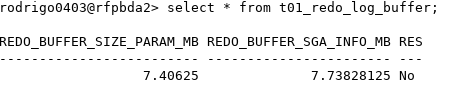
\includegraphics[width=0.7\linewidth]{c1}

\begin{itemize}
  \item Generar una instrucción que muestre la lista de servicios registrados en
    el listener, y explicar, ¿qué valores deberían tener las variables
    established y refused de los dispatchers D000 Y D001?\\
    Tanto \textit{established} como \textit{refused} deberían tener el valor de
    cero debido a que no se ha establecido ni rechazado conexiones. Lo anterior
    debido que los dispatchers se acaban de crear.
\end{itemize}

\section*{C2}

\subsection*{El contenido del script \texttt{s-02-conexiones.sql}}

\lstinputlisting[language=SQL]{\codedir/s-02-conexiones.sql}

\subsection*{El contenido del archivo \texttt{tnsnames.ora}}

\lstinputlisting[language=Bash]{\codedir/c2.ora}

\section*{C3}

\subsection*{El contenido del script \texttt{s-03-consultas.sql}}

\lstinputlisting[language=SQL]{\codedir/s-03-consultas.sql}

\subsection*{El contenido de cada tabla de este script}

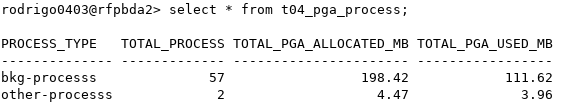
\includegraphics[width=0.9\linewidth]{c3}

\section*{C4}

\subsection*{Respuestas del inciso A: Background y Foreground processes}

\begin{itemize}
  \item Indicar la diferencia entre un background y un foreground process así
    como la forma en la que se puede identificar en la base de datos. \\[3mm]
    Los proces de \textit{background} son procesos que se ejecutan en segundo
    plano para que el Oracle DBMS funcione en sí, mientas que los procesos de
    \textit{foreground} son aquellos que hacen posible que los clientes puedan
    realizar su trabajo (Por ejemplo ejecutar alguna sentencia SQL).
    Los procesos de background suelen ser creados por el listener.\\

    Para reconocer el tipo de proceso existen dos formas. 
    \begin{enumerate}
      \item v\$session.type puede tener el valor de 'BACKGROUND' o 'USER' que
        corresponden a procesos de background y foreground respectivamente.
      \item v\$process.background será null para procesos de tipo foreground y
        tendría valores para procesos de background.
    \end{enumerate}

\end{itemize}

\subsection*{El contenido del script \texttt{s-04-procesos.sql} }

\lstinputlisting[language=SQL]{\codedir/s-04-procesos.sql}

\subsection*{El contenido de cada tabla de este script}

\textbf{Nota}: La columna `B' significa background
\lstinputlisting[language=SQL, basicstyle=\tiny,firstline=6]
  {\codedir/c4.txt}

\subsection*{Las instrucciones que muestran a los 2 procesos del sistema 
  operativo (user y server process)}

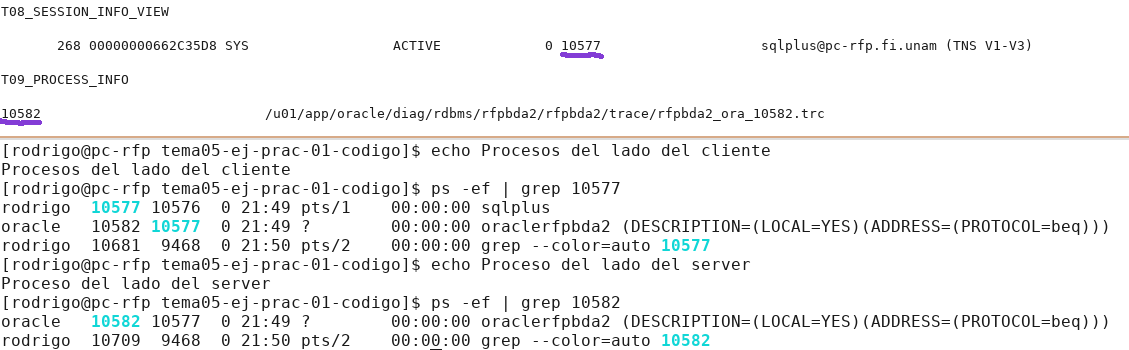
\includegraphics[width=0.8\linewidth]{c4}

\section*{C5. Validador}

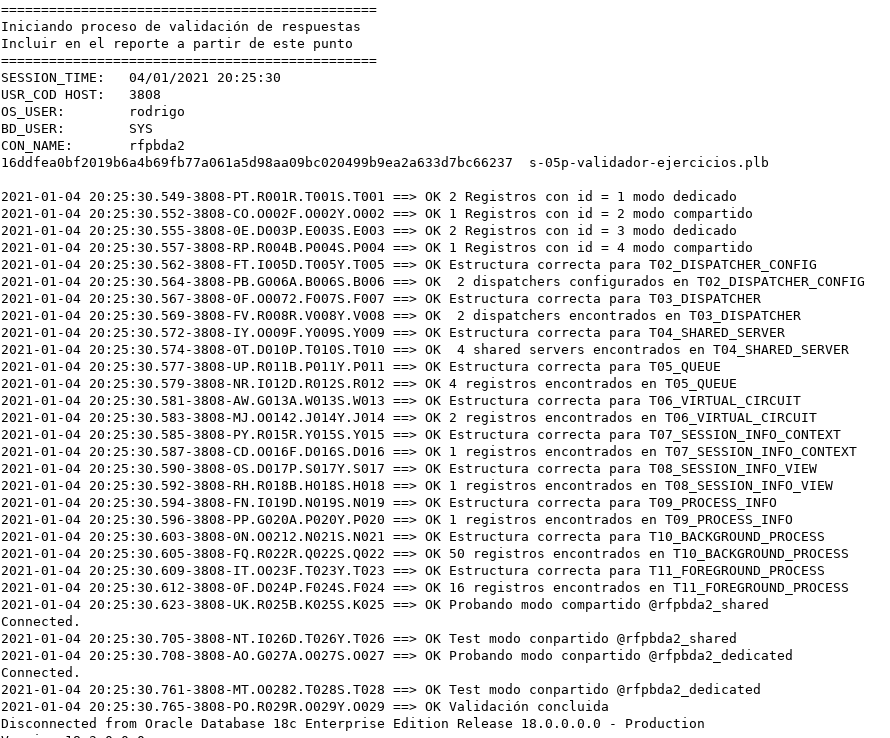
\includegraphics[width=0.8\linewidth]{bda-tema05-ep01-validador}

\section*{Comentarios y conclusiones}

En este ejercicio pusimos en práctica la configuración para modo compartido y
modo dedicado, honestamente cuando se vio de forma teórica pensé que la
configuración sería tardada y algo complicada, si embargo, resultó todo lo
contrario. Basto con configurar algunos parámetros por medio de instrucciones
de tipo \texttt{alter} y configurar el archivo \texttt{tnsnames.ora} con ayuda
de las herramientas que Oracle tiene instaladas.\\

Por otra parte, entendí como se relacionan los procesos del base de datos con
los procesos del sistema operativo. Esto es bastante útil a la hora de que como
DBAs se nos pida cerrar la sesión de un usuario de manera inmediata.

\begin{thebibliography}{99}
    \bibitem{burleson} Burleson Consulting. \textit{Oracle tips } en 
    \texttt{http://www.dba-oracle.com/oracle\_news/}
  \bibitem{oracle} Oracle Help Center. \textit{Database Performance Tuning 
    Guide} en \texttt{https://docs.oracle.com/database/\\%
    121/TGDBA/tune\_buffer\_cache.htm\#TGDBA294}
    % http://www.adp-gmbh.ch/ora/concepts/processes/index.html
\end{thebibliography}

\end{document}
